\documentclass[11pt]{article} \usepackage{mystyle-new}
\usepackage{epsfig,amsmath} \usepackage{graphics}
\usepackage{cite,./mcite}
 
%


% macro for new list environment; defl
  \newcommand{\deflab}[1]{#1\hfil}%
  \newenvironment{defl}[1]%
  {\begin{list}{}{\settowidth{\labelwidth}{#1}%
  \setlength{\leftmargin}{\labelwidth}%
  \addtolength{\leftmargin}{\labelsep}%
  \setlength{\itemsep}{0pt plus 1pt}
  \setlength{\parsep}{0pt plus 1pt}
  \setlength{\topsep}{0pt plus 1pt}
  \setlength{\partopsep}{0pt plus 1pt}
  \setlength{\parskip}{2mm plus 1mm minus 1mm}
  \let\makelabel\deflab}}%
  {\end{list}}
%
%
% User commands may be inserted here:
% ----------------------------------
\newcommand{\Pom}{I$\!$P}                % gives pomeron symbol
\def\lsim{\mathrel{\rlap{\lower4pt\hbox{\hskip1pt$\sim$}}
    \raise1pt\hbox{$<$}}}                % less than or approx. symbol
\def\gsim{\mathrel{\rlap{\lower4pt\hbox{\hskip1pt$\sim$}}
    \raise1pt\hbox{$>$}}}                % greater than or approx. symbol
%
%\newcommand{\cascadeversion}{~2.2.0-beta-0.1}
\newcommand{\cascadeversion}{~\input ../include/casvers-tex.inc}
\newcommand{\cA}{{\cal A}}
\newcommand{\as}{\ensuremath{\alpha_\mathrm{s}}}
\newcommand{\asb}{{\bar \alpha}_\mathrm{s}}
\newcommand{\ga}{\gamma}
\newcommand{\om}{\omega}
\newcommand{\order}[1]{{\cal O}\left(#1\right)}
\newcommand{\tq}{{q}_t}
\newcommand{\tqn}{{q}_{t\;n}}
\newcommand{\Pmax}{\bar{q}}
\def\prp{t}
\newcommand{\kt}{k_{t}}
\def\kti#1{\ensuremath{k_{\prp #1}}}
\def\pti#1{\ensuremath{p_{\prp #1}}}
\def\kt{\ensuremath{k_{\prp}}}
\def\shat{\ensuremath{\hat{s}}}
\newcommand{\pt}{p_{t}}
\newcommand{\ktp}{k_{t}^{\prime}}
\newcommand{\SMALLXC}{SMALLXa,SMALLXb}
\newcommand{\CCFM}{CCFMa,CCFMb,Catani:1989sg,CCFMd}
\newcommand{\BFKL}{BFKLa,BFKLb,BFKLc}
\newcommand{\LDC}{LDCa,LDCb,LDCc,LDCd}
\newcommand{\alphasb}{\bar{\alpha}_s}
\newcommand{\JETSETMC}{\PYTHIAMC}
\newcommand{\LEPTOMC}{Ingelman_LEPTO65}
\newcommand{\PYTHIAMC}{Pythia61}
\newcommand{\RAPGAPMC}{RAPGAP206}
\newcommand{\DGLAP}{DGLAPa,DGLAPb,DGLAPc,DGLAPd}
\def\cascade{{\sc Cascade}}
\def\SMALLX{{\sc Smallx}}
\def\RAPGAP{{\sc Rapgap}}
\def\LEPTO{{\sc Lepto}}
\def\PYTHIA{{\sc Pythia}}
\def\HERWIG{{\sc Herwig}}
\def\JETSET{{\sc Jetset}}
\def\tmdlib{{\sc TMDlib}}
\def\katie{{\sc KaTie}}
\def\powheg{{\sc Powheg}}
\def\madgraph{{\sc MadGraph}}
\def\herwig{{\sc Herwig}}
\def\pythia{{\sc Pythia}}
\def\mcatnlo{{\sc Mc@nlo}}

\def\question#1{\footnote{\textbf{QUESTION: #1}}}
\def\answer#1{\footnote{\textbf{ANSWER: #1}}}
\newcommand{\todo}[1]{\vspace*{3mm}\par\noindent\textbf{\boldmath \Longrightarrow$ #1}\vspace*{4mm}}

\newcommand{\ccfm}{Ciafaloni:1987ur,Catani:1989yc,Catani:1989sg,Marchesini:1994wr}
\newcommand{\bfkl}{Kuraev:1976ge,Kuraev:1977fs,Balitsky:1978ic}
\newcommand{\dglap}{Gribov:1972ri,Lipatov:1974qm,Altarelli:1977zs,Dokshitzer:1977sg}

% Start of document
% -----------------
\makeindex
\begin{document}
%
\begin{flushright}
%DESY 10-107 \\
 Feb 2018
\end{flushright}
\begin{center} {\sffamily\Large\bfseries 
The Monte Carlo generator CASCADE: \\ \vspace*{0.2cm}
LHE interface  and initial state parton showers from TMDs \\ \vspace*{0.2cm}
Version\cascadeversion\  \\  \vspace{0.5cm}}
{ \Large H.~Jung$^{1}$,}\\
      {\large $^1$DESY, Hamburg, FRG}\\
\end{center}
\begin{abstract}
The interface to read in LHE files into the  \cascade\ package is described.
The LHE files can be either files with off-shell initial state  partons, as
generated by the \katie\ package or also files which are generated by 
collinear fixed order calculations like \powheg\ or \madgraph , where a
transverse momentum of the initial state partons is added according to the
appropriate transverse momentum dependent (TMD) parton distribution.
\end{abstract} 
\newpage
{\sffamily\large\bfseries PROGRAM SUMMARY} \\ \\
{\em Title of Program:} \cascade\ \cascadeversion\ \\ \\
{\em Computer for which the program is designed and others on which it is
operable:}   any with standard Fortran 77 (g77 or gfortran), tested on 
                 SGI, HP-UX, SUN, PC, MAC\\ \\
{\em Programming Language used:}  FORTRAN 77 \\ \\
{\em High-speed storage required:}  No \\ \\
{\em Separate documentation available: } No \\ \\
{\em Keywords: } QCD, TMD parton distributions.\\ \\
\\ \\
{\em Method of solution:}  
Since measurements involve complex cuts and multi-particle final states, the 
ideal tool for any theoretical description of the data is a Monte Carlo 
event generator which generates initial state parton showers according to Transverse Momentum Dependent (TMD) parton densities, in a backward evolution. The evolution follows the DGLAP evolution equation exactly as used for the determination of the TMD. \\ \\
{\em Restrictions on the complexity of the problem:}  
Any LHE file (with on-shell or off-shell) initial state partons can be processed.\\ \\
{\em Other Program used:}  \PYTHIA\ ({\it version $>$ 6.4}) for hadronization, 
\tmdlib\ as a library for TMD parton densities 
{\sc Bases/Spring}  5.1 
for integration (supplied with the program package).\\ \\ 
%{\em Download of the program:} \verb+http://projects.hepforge.org/cascade/+
{\em Download of the program:} \verb+http://www.desy.de/~jung/cascade+\\ \\
{\em Unusual features of the program:}   None \\ \\
\newpage

%======================================================================

\section{Introduction}

In recent years the simulation of processes at the LHC has been often separated into two parts,
the precision calculation of the hard process at higher order in the strong coupling $\alpha_s$ at
next-to-leading (or even higher) order as implemented in packages like \powheg\ ~\mcite{Alioli:2010xa,Frixione:2007vw} or \mcatnlo\ ~\mcite{Frixione:2006gn,Frixione:2003ei,Frixione:2002bd,Frixione:2002ik} or 
\herwig\, and the simulation of the subsequent parton radiation in form of parton showers and 
hadronization and multiparton interaction, which is then performed by \pythia\ or \herwig .  
The interface between both parts is the so-called 
Les Houches Event (LHE) file~\cite{Alwall:2006yp}, which contains all the information of the hard process including the
color structure.  

With the developments
in determination of transverse momentum dependent (TMD) parton densities  \cite{Hautmann:2017fcj,Hautmann:2017xtx}, it is natural to
develop a scheme, where the initial parton shower follows exactly the TMD parton density and 
where either collinear (on-shell) of \kt-dependent (off-shell) hard process calculations can be
combined. The Monte Carlo event generator \cascade\ \mcite{Jung:2010si,Jung:2001hx,Jung:2000hk} is used for this, since it provides already
a frame to perform initial state parton showers following the un-integrated gluon density. 
In this report we describe, how this frame can be extended to include all flavors in the parton shower
and how the hard process can be used via LHE files.

\section{The hard process}
\label{sec:LHEfiles}

The hard process is generated externally either with \powheg ~\mcite{Alioli:2010xa,Frixione:2007vw} with on-shell kinematics or with \katie ~\cite{vanHameren:2016kkz} with off-shell kinematics for the initial state partons. The events from the hard process are read into the \cascade\ package via LHE files.

For processes generated with \katie\ no further corrections need to be performed and the event can be directly
passed to the showering procedure, described in the next section.

For processes with collinear kinematics of the initial state partons, a transverse momentum is added, according to the 
TMD parton density, however, care has to be taken, that energy and momentum is still conserved. The procedure is the following:
for each initial parton, a transverse momentum is assigned according to the TMD density, and this system is rotated and booted to its center-of-mass frame. Since the initial state partons have transverse momentum, they acquire a virtuality. The energy and longitudinal component of the initial momenta are recalculated taken this virtuality into account, by \cite{Bengtsson:1986gz}:
\begin{eqnarray}
E_{1,2} &=& \frac{1}{\sqrt{2\shat}} \left( \shat \pm (Q_2^2 - Q_1^2) \right)\\
p_{z\;1,2} & = &  \pm \frac{1}{2\sqrt{\shat}}\sqrt{(\shat + Q_1^2 +Q_2^2)^2 - 4Q_1^2Q_2^2 }
\end{eqnarray}
where $Q_1^2$ and $Q_2^2$ are the virtualities of parton $1,2$ after the transverse momentum is assigned.
The final partons of the hard system are rotated and boosted to it's center-of-mass frame. 
Then the whole system of initial and final state partons is boosted and rotated back to its original system. This procedure is similar to the procedure applied in standard parton showers like \pythia , when a transverse momentum is created from the shower. The difference here is, that the transverse momentum is taken from the TMD directly, and the initial state shower will not change this anymore.

 \section{Initial State Parton Shower based on TMDs}
\label{TMDshower}
The parton shower, which is described here, follows consistently the parton evolution of the TMDs. 
By this we mean that the splitting functions $P_{ab}$, the order in \as , the scale in the calculation of \as\, as well as the kinematic restrictions applied are identical in both the parton shower and the evolution of the parton densities.

A backward evolution method, as now common in Monte Carlo event generators, is applied for the initial state parton shower, evolving from the large scale of the matrix-element process backwards down to the scale of the incoming hadron. However, in contrast to the conventional parton shower, which generates a transverse momentum of the initial state partons during the backward evolution, the transverse momentum of the initial partons of the hard scattering process is fixed by the TMD and the parton shower does not change the kinematics.
The transverse momenta during the cascade follow the behavior of the TMD.  The hard scattering process is obtained directly using off-shell matrix element calculations as described in section~\ref{sec:LHEfiles}. 

The backward evolution of the initial state parton shower follows very closely the description in \mcite{Bengtsson:1986gz,Jung:2010si,Jung:2001hx,Jung:2000hk}. The evolution scale $\mu$ is selected from the hard scattering process, with $\mu^2 = \hat{p}_T^2$  or $\mu^2 = Q_t^2 +\hat{s}$ for an evolution in virtuality or angular ordering, with $\hat{p}_T$ being the transverse momentum of the hard process, $Q_t$ being the vectorial sum of the initial state transverse momenta and $s$ being the invariant mass of the subprocess.  

Starting with the hard scale $\mu=\mu_{i}$, the  parton shower algorithm searches for the next scale $\mu_{i-1}$ at which a resolvable branching occurs. This scale $\mu_{i-1}$ is selected from the Sudakov form factor $\Delta_S$ making use of the TMD densities $\cA_a(x',\kt',\mu')$ which depend on the longitudinal momentum fraction $x'=x z$ of parton $a$, its transverse momentum $\kt'$ probed at a scale $\mu'$ (see also \cite{Jung:2010si}). The Sudakov form factor $\Delta_S$ for the backward evolution is given by (see fig.~\ref{parton-branching} left):
\begin{equation}
\Delta_S(x,\mu_{i},\mu_{i-1}) = \exp\left[ - \int_{\mu_{i-1}}^{\mu_{i}} \frac{d \mu'}{\mu'} \frac{\as({\tilde \mu'})}{2 \pi} \sum_a \int dz P_{a\to bc}(z) \frac{x'\cA_a(x',\kt',\mu')}{x\cA_b(x,\kt,\mu')} \right]
\label{sudakov}
\end{equation}
which describes the probability that parton $b$ remains at $x$ with transverse momentum $\kt$ when evolving from $\mu_i$ to $\mu_{i-1} < \mu$. Please note, that the argument in \as\ is $\tilde \mu'$ and depends on the ordering condition as discussed later.
\footnote{In equation eq.(\ref{sudakov}) ordering in $\mu$ is assumed, if  angular ordering, as in CCFM~\cite{\ccfm}, is applied then the ratio of parton densities would change to $ \frac{x'\cA_a(x',\kt',\mu'/z)}{x\cA_b(x,\kt,\mu')}$ as discussed in \cite{Jung:2010si}.}

In the parton shower language, the selection of the next branching comes from solving the Sudakov form factor eq.(\ref{sudakov}) for $\mu_{i-1}$.
However, to solve the integrals in eq.(\ref{sudakov}) numerically for every branching would be too time consuming, instead the veto-algorithm \cite{Bengtsson:1986gz,Platzer:2011dq} is applied. The selection of $\mu_{i-1}$ and the branching splitting $z_{i-1}$ follows the standard methods \cite{Bengtsson:1986gz}. 

The splitting function $P_{ab}$ as well as the argument $\tilde \mu$ in the calculation of \as\ is chosen exactly as used in the evolution of the parton density. In a parton shower one treats ``resolvable'' branchings, defined via a cut in $z < z_M$ in the splitting function  (see eq.(\ref{eq:Tg})) to avoid the singular behavior of the terms $\frac{1}{1-z}$, and branchings with $z> z_M$ are regarded as ``non-resolvable'' and are treated similarly as virtual corrections: they are included in the Sudakov form factor $\Delta_S $. 

\begin{figure}[htb]
\begin{center} 
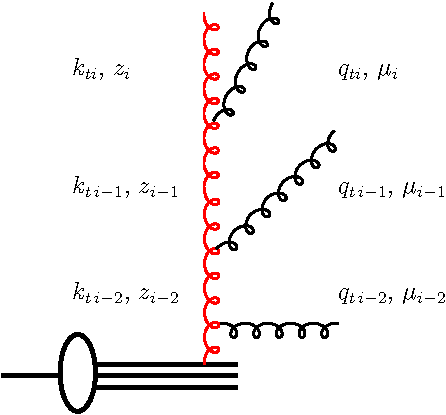
\includegraphics[width=0.25\textwidth]{parton-shower-evolution-crop} \hskip 2cm
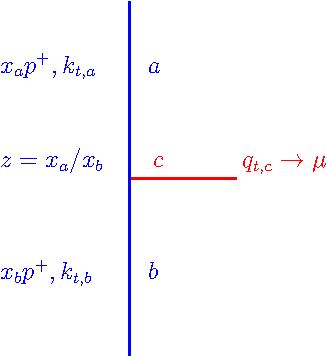
\includegraphics[width=0.2\textwidth]{splitting-process-latex-crop} 
  \caption{Left: Schematic view of a parton branching process. Right: Branching process $ b \to a + c$.}
\label{parton-branching}
\end{center}
\end{figure} 

The longitudinal momentum fraction $x_{i-1}= \frac{x_i}{z_{i-1}}$ is calculated by generating $z_{i-1}$ according to the splitting function. With $z_{i-1}$ and $\mu_{i-1}$ all variables needed for a collinear parton shower are obtained. 

The calculation of the  transverse momentum $\kt$ is sketched in fig.~\ref{parton-branching} right.
The transverse momentum $q_{t\,i}$ can be  obtained by giving a physical interpretation to the evolution scale $\mu_i$ (see fig.~\ref{parton-branching} right), and $q_{t\,i}$ can be calculated in case of angular ordering ($\mu$ is associated with the angle of the emission)  in terms of the angle $\Theta$ of the emitted parton wrt the beam directions $q_{t,c} = (1-z) E_{b} \sin \Theta$:
\begin{equation}
  \label{ang-ordering}
 {\bf q}_{t,i}^2  =  (1-z)^2 \mu_i^ 2  \;\; .
\end{equation}

Once the transverse momentum of the emitted parton $q_t$ is known, the transverse momentum of the propagating parton can be calculated from
\begin{equation}
{\bf k}_{t\,i-1} = {\bf k}_{t\,i} + {\bf q}_{t\, i-1}
\end{equation}
with a uniformly distributed azimuthal angle $\phi$ is assumed for the vector components of $\bf k$ and $\bf q$.

The whole procedure is iterated until one reaches a scale $\mu_{i-1} < q_0$ with $q_0$ being a cut-off parameter, which can be chosen to be the starting evolution scale of the TMD. However, it turns out that during the backward evolution the transverse momentum $k_t$ can reach large values, even for small scales $\mu_{i-1}$, because of the random $\phi$ distribution. On average the transverse momentum decreases, and it is of advantage to continue the parton shower evolution to a scale $q_0 \sim \Lambda_{qcd} \sim 0.3$~GeV, to allow enough emissions to share the transverse momenta generated.


%----------------------------------------------------------------------
\subsection{The TMD parton density}

In the previous versions of \cascade\ the TMD densities where part of the program. With the development of \tmdlib ~\cite{Hautmann:2014kza} 
there is easy access to all available TMDs, they can be selected, as before, via \verb+IGLU+ with a value $>100000$.
For example the TMDs from the parton branching method \cite{Hautmann:2017fcj,Hautmann:2017xtx} are selected via  \verb+IGLU=101600+ or the ones from the KMR approach,
as used in are selected via  \verb+IGLU=410000+ as in Ref.~\cite{Bury:2017jxo}


%%%%%%%%%%%%%%%%%%%%%%%%%%%%%%%%%%%%%%%%%%%%%%%%%%%%%%%%%%%%%%%%%%%%%%%%%%

\subsection{$\alpha_s$}
%%%%%%%%%%%%%%%%%%%%%%%%%%%%%%%%%%%%%%%%%%%%%%%%%%%%%%%%%%%%%%%%%%%%%%%%%%
The strong coupling $\alpha_s$ is calculated via the \PYTHIA~\cite{\PYTHIAMC}  subroutine \verb+PYALPS+. 
Maximal and minimal number of flavours used in $\alpha_s$ are set by
\verb+MSTU(113)+ and \verb+MSTU(114)+, $\Lambda_{QCD}$ = \verb+PARU(112)+ with respect to the number of flavours given in
\verb+MSTU(112)+ .


\subsection{Final state parton showers}



%The gluons emitted in the initial state can undergo further timelike branchings. The maximum timelike mass $m_{max}$ is calculated using the angular constraint. With this mass, the parton which can further undergo a timelike branching is boosted to its rest frame with $m_{max}$ but keeping the original energy. The timelike branching is performed with the \PYTHIA\ routine \verb+PYSHOW+. After successful timelike branching, the proper mass is associated to the parton and the kinematics are calculated appropriately.

The final state parton shower uses the parton shower routine \verb+PYSHOW+ 
of \PYTHIA\
with the default scale $\mu^2=2\cdot (m_{1\;\perp}^2+m_{2\;\perp}^2)$ (\verb+IFIN=1+),
with $m_{1(2)\;\perp}$ being the transverse mass of the hard parton 1(2). Other choices are possible: $\mu^2=\hat{s}$ (\verb+IFIN=2+) and $\mu^2=2\cdot (m_1^2+m_2^2)$ (\verb+IFIN=3+). 
Relevant for processing LHE files is the scale \verb+SCALUP+ provided from the hard scattering process. This scale can be used for final state parton shower with \verb+IFIN=4+
In addition a scale factor can be applied: \verb+SCAF+$\times\mu^2 $ (default:  \verb+SCAF=1+).



\section{Description of the program components}
In \cascade\ all variables are declared as \verb"Double Precision". The 

The program has to be compiled and linked together with \PYTHIA\ 6, to ensure that the double
precision code of \JETSET\  is loaded.

When \verb+HEPMC+ is included, the output of \cascade\ is a standard HEPMC~\cite{Dobbs:2001ck} file, which can be further processed
for example with Rivet \cite{Buckley:2010ar}. 


\subsubsection{Parameters}
\begin{defl}{123456789012345}
\item[{\tt NEVENT:}] number of events to be processed, for NEVENT = -1 all event in the LHE file are read.
\item[{\tt IPRO:}]                  =-1  read LHE file
\end{defl}
\subsubsection{Parameters for parton shower and fragmentation}
\begin{defl}{123456789012345}
\item[{\tt NFRAG:}] \index{NFRAG} (D: = 1)
                        switch for fragmentation 
\item[] = 0: off
\item[] = 1: on 
\item[{\tt IFPS:}] \index{IFPS} (D: = 3)
                  switch for parton shower .
\item[] = 0: off
\item[] = 1: initial state
\item[] = 2: final state
\item[] = 3: initial and final state  
\item[{\tt ITIM:}] \index{ITIM} (D: =1)
\item[] =0: no shower of time like partons
\item[] =1: time like partons may shower
\item[{\tt ICCFM:}] \index{ICCFM} (D: =1)
\item[] =0: DGLAP type evolution (one loop, old version)
\item[] =1: CCFM evolution (all loops)
\item[] =2: full flavor TMD parton shower with DGLAP splitting function. No upper cut on \kt in shower applied
\item[] =3: full flavor TMD parton shower with DGLAP splitting function with upper cut on \kt of shower given by \kt of off-shell initial partons
\item[{\tt IFIN}] \index{IFIN} (D:=1)  scale switch for  final state parton shower
\item[] = 1: $\mu^2=2 (m^2_{1\;t} + m^2_{2\;t})$
\item[] = 2: $\mu^2=\hat{s}$
\item[] = 3:  $\mu^2=2 (m^2_{1} + m^2_{2})$
\item[] = 4:  2*\verb+SCALUP+

\item[{\tt SCAF}]\index{SCAF} (D:=1.) scale factor for final state parton shower
\end{defl}

\subsubsection{Parameters for parton densities}
\label{sec:alphas}
\begin{defl}{123456789012345}
\item[{\tt IGLU:}] \index{IGLU} (D: = 1201)
			select TMD parton density
\item[]   $> 100000$:  call \tmdlib\ for TMD densities
\item[]  \verb+IGLU=410000+ BHKS TMD \cite{Bury:2017jxo}
\item[]  \verb+IGLU=101600+ parton branching TMD \cite{Hautmann:2017fcj}
\end{defl}

\subsubsection{Parameters for LHE files}
\label{sec:lhe}
\begin{defl}{123456789012345}
\item[{\tt CLHE}]  name of LHE file
\item[{\tt ITMW}]  =0:  LHE file has off shell initial partons
\item[] = 1: generate \kt according to TMD given with IGLU and change initial on-shell partons
\item[] = 2: same as =2, but reweight also to TMD given with IGLU but with fact.scale
\end{defl}


%   
\section{Program Installation}
\cascade\ now follows the standard AUTOMAKE
convention. To install the program, do the following
\begin{tiny}
\begin{verbatim}
1) Get the source

tar xvfz cascade-XXXX.tar.gz
cd cascade-XXXX

2) Generate the Makefiles (do not use shared libraries)
./configure --disable-shared --prefix=install-path --with-pythia6="pythia_path"  --with-lhapdf="lhapdflib_path" 
--with-tmdlib="TMDlib-path" --with-gsl="gsl_lib" --with-hepmc="hepmc_path"

with (as example):
pythia_path=/afs/desy.de/group/alliance/mcg/public/MCGenerators/pythia6/422/i586_rhel40
lhapdflib_path=/afs/desy.de/group/alliance/mcg/public/MCGenerators/lhapdf/5.8.1/i586_rhel40

3) Compile the binary
make

4) Install the executable and PDF files
make install 

4) The executable is in bin
run it with:
export CASED=1242425
export HEPMCOUT=outfile.hepmc

cascade < steer_pp-LHEin

\end{verbatim}
\end{tiny}
%\section{Acknowledgments}
%We are very grateful to B.~Webber for providing us with the \SMALLX~
%code, which was the basis for the \cascade\ Monte Carlo generator.  
%We are very grateful also to G.~Ingelman and T.~Sj\"ostrand for many discussions and for their courtesy to let us use their code for proton remnant treatment.
 

\bibliographystyle{heralhc} 
\raggedright 
%\bibliography{/Users/jung/Bib/hannes-bib}
\input cascade-lhe.bbl
\end{document} 





